This section will look at how ML-Agents\footnote{\url{https://github.com/Unity-Technologies/ml-agents}} can be used to create machine learning models for the vehicles and the pedestrians. ML-Agents is an open-source project designed to train agents using reinforcement learning and imitation learning. The purpose of this is to allow users to have multiple entities in the scene without controlling all of them. ML-Agent is both imported as an addon to Unity, but it also runs as a separate Python library. When the simulator starts, Unity would then open a port to communicate with Python. 

For this project, the hope was to simulate the interaction between the different forms of traffic. However, creating and uploading the simulator onto an external server to train can take a long time. The priority was therefore to train a model for the vehicles. This was done by first training on one vehicle and then looking at collaboration learning.  As will be discussed in chapter~\ref{results}, the vehicles have mixed results and time was spent trying to improve this rather than developing the pedestrians further. The ML training scripts can simply be attached to the pedestrians as shown in figure~\ref{06:fig:MLMap4}.  

\subsection{Network Model}
A variety of different model designs have been attempted throughout this project. This section will look at what decisions were made and why that was the case. More information on the tuning can be found in Chapter~\ref{results}.

\subsubsection{Model inputs}
The first thing to look at is the inputs to the model. The common way when looking online for making autonomous vehicles using ML-Agents is to use checkpoints that span the road. The vehicles would then learn to drive towards the checkpoint and away from the walls. The reason why this would not work for this project is that the rays get blocked by the checkpoint. If there is a pedestrian or a car on the other side the vehicle will not observe them. The solution was instead to guide the vehicles in the direction they should drive. The vehicle is therefore given the angle between its direction and the vector going to the target. This was done by using the calculate angle command in Unity which only returns positive values. For the vehicle to know which way to turn, a simple calculation was made where if the target was on the left the angle would be multiplied by -1. The input angle was then scaled to be between -1 and 1. 

To further increase the performance, the angle was passed through different scaling functions. This can be seen in Figure~\ref{06:anglePlot}. The reason for doing this was to strengthen the input single for smaller angles. This would improve the performance for two reasons. Firstly, as the car cannot turn more than 60 degrees the input angle could be scaled in such a way that for larger angles the input would be close to 1. Passing the input angle through a tanh function strengthens the sensitivity for smaller angles. Therefore, the vehicles use $tanh(2.5x/180)$ where x is the angle. 

\begin{figure}[h]
    \centering
    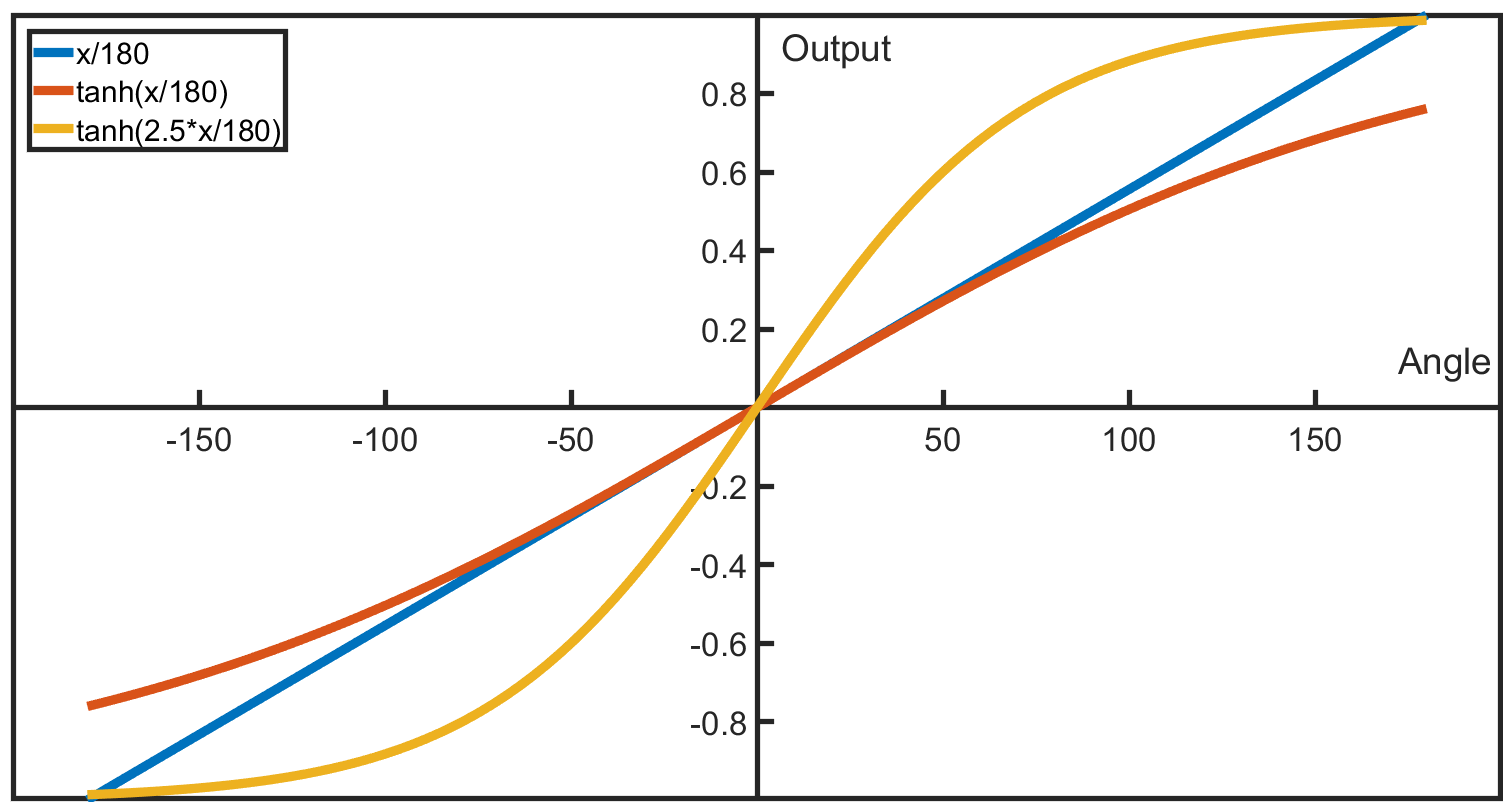
\includegraphics[width=0.8\textwidth]{06_Implementation/00_MLAgents/Images/anglePlot.png}
    \caption[Input angle functions]{The plot shows different functions applied to the input angle. The aim of using $tanh(2.5x/180)$ is that it decreases the change for larger angles, but increase for smaller.} \label{06:anglePlot}
\end{figure}


For the sensing APIs, the options are either to use raycasts or to use a camera sensor. The advantage of using raycasts is that network does not have to be as complex as for the image processing. Another advantage is that when building the simulator as a server build, enabling the rendering is slightly complicated and decreases the speed of the simulator. The advantage of using the camera sensor is that it can more accurately simulate the real environment as a complex network could distinguish what the camera is capturing.  In Unity, this is not needed as the rays can distinguish what type of object it is detecting. However, in the real world, this is impossible. The next step would be to calculate how many inputs from the raycasts there will be. The 3D rays come with several configurations\footnote{\url{https://github.com/Unity-Technologies/ml-agents/blob/main/docs/Learning-Environment-Design-Agents.md#raycast-observations}} such as the number of rays per direction, max ray degrees, detectable tags and observation stacking. The total size of the created observations is $(Observation Stacks) * (1 + 2 * Rays Per Direction) * (Num Detectable Tags + 2)$. Observation stacking can be used to give the network a limited short term memory. This is done by repeating observations from previous steps. For example, if the input from a sensor was
\begin{equation}
  \begin{aligned}
   step 1: 0.1\\
step 2: 0.2\\
step 3: 0.3\\
step 4: 0.4
\end{aligned}
\end{equation}
then the stacked input would then look something like this:
\begin{equation}
  \begin{aligned}
step 1: [0.1, 0.0, 0.0]\\
step 2: [0.2, 0.1, 0.0]\\
step 3: [0.3, 0.2, 0.1]\\
step 4: [0.4, 0.3, 0.2]\\
\end{aligned}
\end{equation}

Changing observation stacking made very little difference to the performance of the network, so this value was left at 1.

The next two values to decide was the number of rays per direction and the spread of these rays. Ideally, the agent should use as few as possible whilst at the same time having good coverage of the surrounding area. When using too many inputs, the model was had difficulty figuring out where to drive as the signals from the ray sensors would overpower the one pointing the direction. The best result was found with about 6 rays per direction and an angle of 120 degrees. This would be a total of 13 sensors as one is pointing forward. The angle is wide enough so that if an entity comes from behind the vehicle would know not to turn into it. To compensate for fewer sensors the ML agents use a sphere cast rather than a ray cast. This means that the detection area is much larger than a single point. This will help detect pedestrians as can be seen in Figure~\ref{06:fig:MLMap4}. This limits the probability of the pedestrians ending up being between two rays.  

The last input that was given to the model was speed so that the model would have some understanding of its momentum. Ideally, the vehicle would use this to control how much braking was necessary. 

\begin{figure}[h]
    \centering
    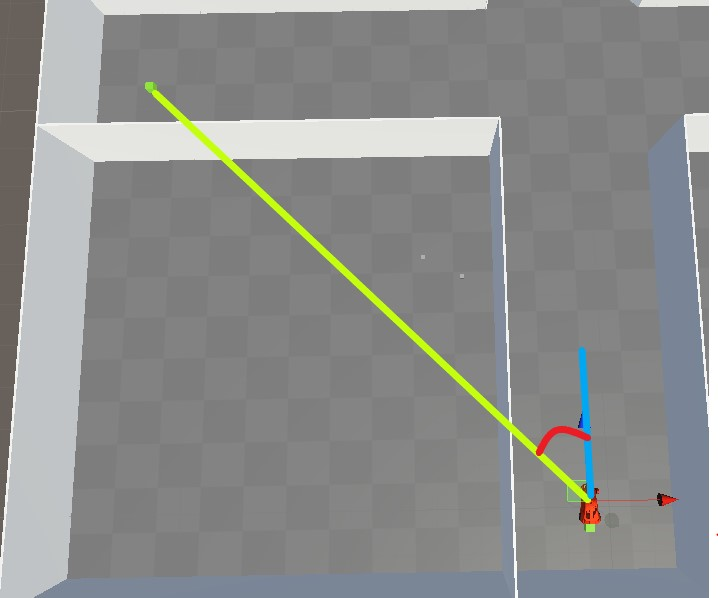
\includegraphics[width=0.8\textwidth]{06_Implementation/00_MLAgents/Images/angle.jpg}
    \caption[Angle visualisation]{The input angle to the model is the angle between the forward vector and the vector going from the vehicle to the target.} \label{06:angleDrawing}
\end{figure}

\subsubsection{Model outputs}
The output of the model matches the vehicle controls. Therefore, The output consists of two values, one for the throttle and breaking and one for turning. The main design decision that had to be made was whether to discrete or continuous output values. Chapter~\ref{results} will look further into this, but basically discrete values work better. This is because the vehicle speed grows with the square root of the input value. Discrete values worked therefore better as they produce strong decisions. 


% Inputs to the model, angle, speed and sensors. Different sensor styles, stack input, sphare cast. Why not camera. 

% Discussion of what the outputs of the network. Choose discrete.

% Why learning by demonstration had to be used as without it took to long for basic behavior

% Network configurations

% Using GAIL and 

\subsection{Learning Environments}
When training using reinforcement learning it is important to have a good environment. Four different environments were used with increasing complexity. To help improve the robustness of the models, the start position and rotation would vary slightly between runs. 

The first map (Figure~\ref{06:fig:MLMap1}) was designed to help the agents learn to drive forward and turn. Every corner had a checkpoint where they received a reward. The issue with this map was that there was not enough randomness, so the map was straightforward no matter where the agent started. 

The second map (Figure~\ref{06:fig:MLMap2}) was a more complex map where the agents would have to turn both left and right with different amounts as they drove around. When training on this map the checkpoint order would flip every other run. This decreased the vehicle performance on this map but increased the robustness. 

The final training map (Figure~\ref{06:fig:MLMap3}) was designed as an intersection where the vehicles would have to navigate around each other to avoid a collision. Up to four vehicles would spawn in one of the checkpoints positions and then drive to a different one. The map was designed in such a way that vehicles would have to wait for each other if they were both going to the same location. 

\begin{figure}[!htbp] 
\centering
\begin{minipage}[t]{.45\textwidth}
\centering
\begin{subfigure}{\textwidth}
        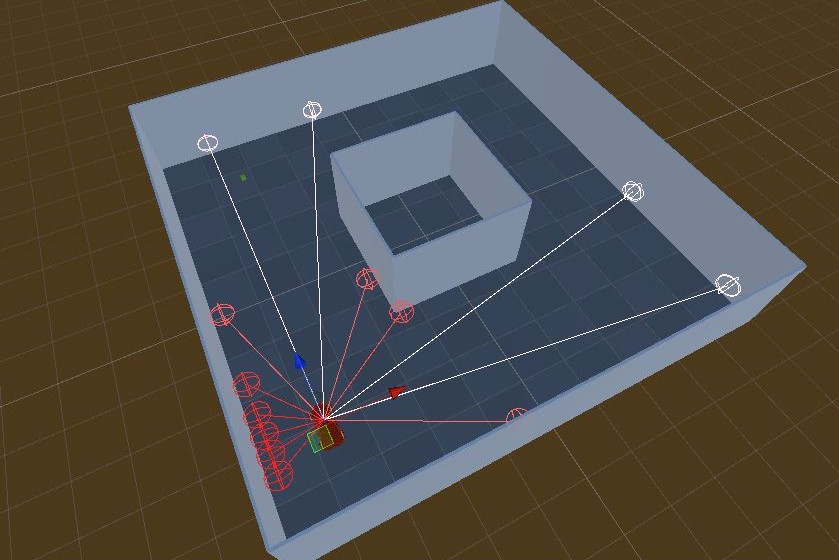
\includegraphics[width=\linewidth, left]{06_Implementation/00_MLAgents/Images/MLMap1.JPG}
        \caption[Training environment map 1]{Simple training environment for the vehicles to drive around.}
        \label{06:fig:MLMap1}
    \end{subfigure}
\end{minipage}
\qquad
\begin{minipage}[t]{.45\textwidth}
    \centering
    \begin{subfigure}{\textwidth}
        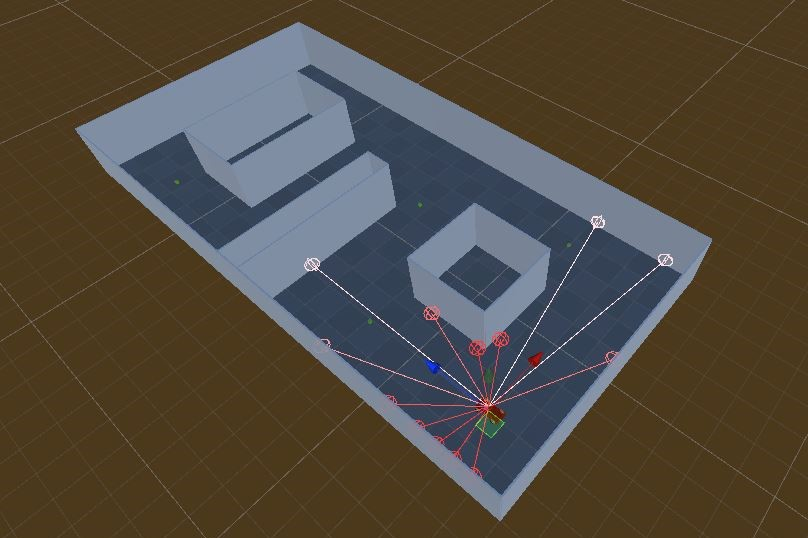
\includegraphics[width=\linewidth, right]{06_Implementation/00_MLAgents/Images/MLMap2.JPG}
        \caption[Training environment map 2]{A slightly more complex map where the vehicles would have to do both left and right turns.}
        \label{06:fig:MLMap2}
    \end{subfigure}
\end{minipage}
\end{figure}

\begin{figure}[!htbp] 
\centering
\begin{minipage}[t]{.45\textwidth}
\centering
\begin{subfigure}{\textwidth}
        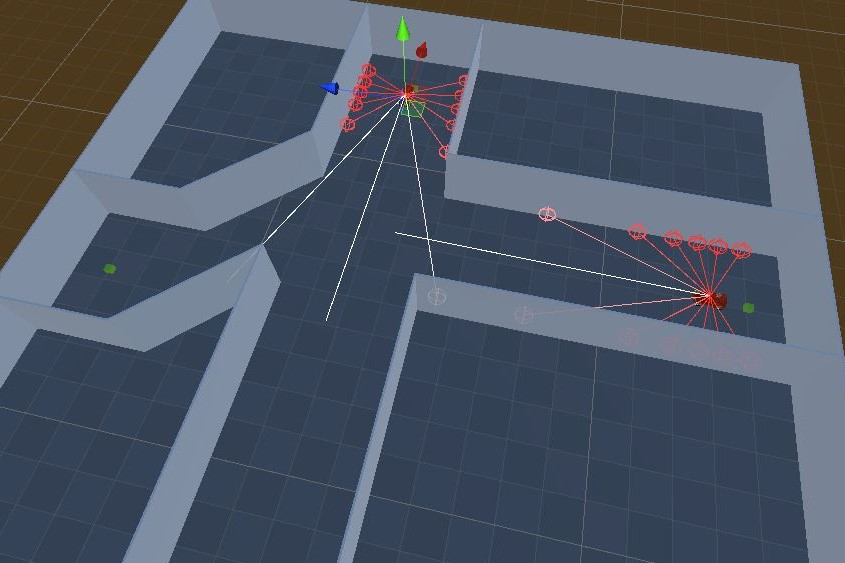
\includegraphics[width=\linewidth, left]{06_Implementation/00_MLAgents/Images/MLMap3.JPG}
        \caption[Training environment map 3]{An intersection map to help the collaboration learning. }
        \label{06:fig:MLMap3}
    \end{subfigure}
\end{minipage}
\qquad
\begin{minipage}[t]{.45\textwidth}
    \centering
    \begin{subfigure}{\textwidth}
        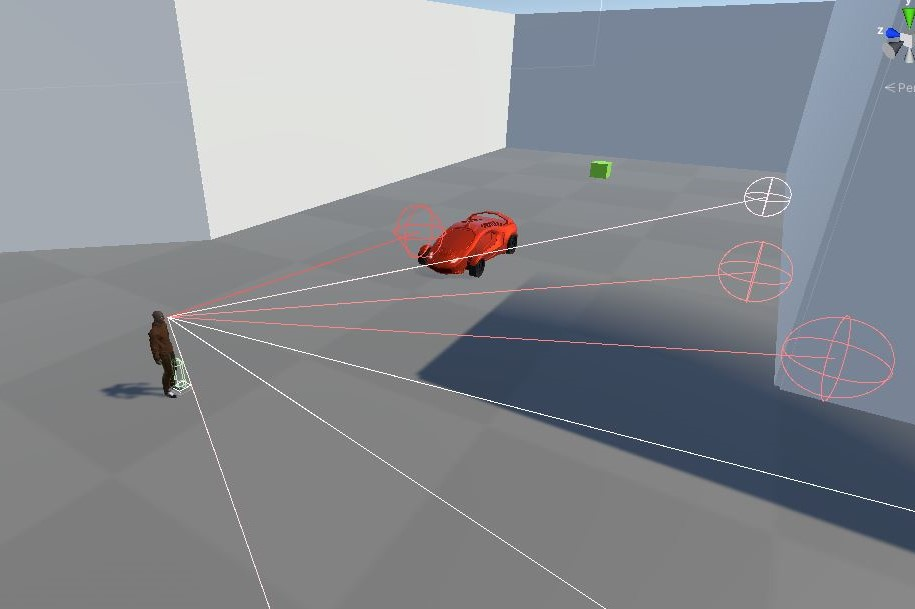
\includegraphics[width=\linewidth, right]{06_Implementation/00_MLAgents/Images/MLMap4.JPG}
        \caption[Training pedestrians]{Intersection map where a pedestrian meets a vehicle.}
        \label{06:fig:MLMap4}
    \end{subfigure}
\end{minipage}
\end{figure}


\subsection{Game controller}
The game controller controls the learning environment. When the episode starts, the controller will spawn the vehicle in a random location with a random target. The controller keeps track of how long the episode has gone on and aborts the training if it takes too long. The controller will then reset the map and spawn a new vehicle in a random position. If a vehicle reaches its target, or if it collides with the wall, the game controller would remove that vehicle from the scene.

The game controller is also responsible for giving team rewards for collaboration learning. This will be explained further in Section~\ref{reward}.

\subsection{Learning by Demonstration} \label{lbd}
Learning by demonstration is used to help the agents learn faster. This is also known as imitation learning. This is done by recording some test runs which the agents would then try to replicate. Imitation learning has been crucial for this project as without it the agents never built up enough momentum to move. When using continuous output values the agents never figured out that holding down forward over a longer time would gain momentum. This was because the reward was only given when the agent moved towards the target. ML-Agents supports learning from demonstration by using Generative Adversarial Imitation Learning (GAIL). GAIL works by creating a second neural network that will try to learn if the observed behaviour is produced from a demonstration or from the agent. If the GAIL network guesses incorrectly the vehicle model receives a reward. This can be computationally slower than other options as two networks are being trained at once. 

Alongside GAIL behaviour cloning can be used. BC aims to train the network in such a way that it will mimic the behaviour from the demonstration files. Behaviour cloning cannot generalise past the examples shown in the demonstration, but together with GAIL it often produces results than without as can be seen in figure~\ref{06:bc}. 

\begin{figure}[h]
    \centering
    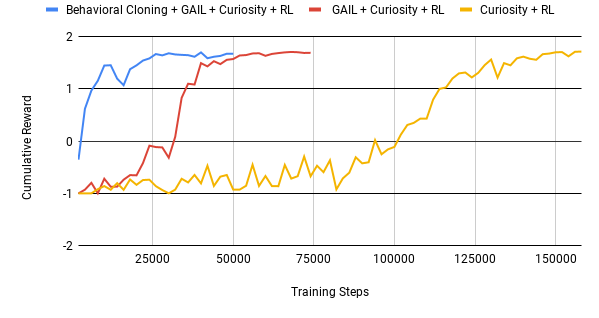
\includegraphics[width=0.9\textwidth]{06_Implementation/00_MLAgents/Images/mlagents-ImitationAndRL.png}
    \caption[Imitation and RL]{The figure shows that using BC and GAIL decreases the number of training steps it takes to train the model.} \label{06:bc}
    \source{\url{https://github.com/Unity-Technologies/ml-agents/blob/0.15.0/docs/Training-Imitation-Learning.md}}
\end{figure}


\subsection{Rewards and Collaboration Learning} \label{reward}
This section will look at the reward system implemented and how that affects collaboration learning. The reward system changes as the vehicles improved. In the early stages, a reward was given when the vehicles moved forwards. Gradually increasing the difficulty is called Curriculum Learning. The agents were also given an additional reward if they faced in the direction of the target. Eventually, this simple behaviour was not needed as later learning was based on this initial model. Currently, vehicles receive a reward every time they reduce the distance between themselves and the target. This caused the vehicles to understand that driving directly towards the target is not necessarily the optimal solution. The vehicles received a large reward when the target was reached and received a large penalty if it collided into the wall. A small penalty was also given every time step to reward faster completions.

For collaboration learning the reward system is slightly different. MA-POCA (MultiAgent Posthumous Credit Assignment) can be used to give team rewards as well as individual rewards. This will teach the agents to work together. When using collaboration learning teams received a reward every time a vehicle reached its target but received a negative reward if a collision occurred. MA-POCA can also be used to train teams against each other. This feature will not be used for this project. 

\subsection{Training}
This part will coverer how training with ML-Agents works. Hyperparameter tuning will be discussed in Section~\ref{MLPreformance}. ML-Agent supports several kinds of models, but for this project, Proximal Policy Optimisation (PPO) and MultiAgent Posthumous Credit Assignment (MA-POCA) is used\cite{MLagentsoverview}.  

\subsubsection{Models}
For individual learning, PPO or Soft Actor-Critic were considered. PPO is shown to be more general-purpose and stable than SAC\cite{FoersterNFTKW17}. SAC uses learn experiences to train. The experiences are placed in a replay buffer which it randomly selects from during training. PPO however learns directly from the environment. SAC is better designed for slower environments, so an autonomous vehicle would be too fast for it. PPO was therefore used for this first part. 

For collaboration learning MA-POCA. This was described in Section~\ref{reward}. When training only one vehicle the episode would end as soon as either the vehicle reached the destination or it collided with the wall. If there were several vehicles in the scene having the whole episode end if one vehicle collided with the wall seemed illogical, as it would make it too hard for the other vehicles to learn. The solution is therefore to only remove the vehicle which collided or reached the target. POCA is designed in such a way that even removed vehicles still receive additional team rewards.   

\subsubsection{Improvements}
Curiosity\footnote{\url{https://github.com/Unity-Technologies/ml-agents/blob/main/docs/ML-Agents-Overview.md#curiosity-for-sparse-reward-environments}} was also tried. Curiosity allowed for random rewards to help the network explore different options.

As mentioned in Section~\ref{lbd}, GAIL and BC were used to help speed up the training by replicating the saved demonstrations. 

\subsubsection{Environments}
There are two ways of speeding up the training. The first one is to create multiple instances of the learning environment (Figure~\ref{06:trainingScene}). This allows several agents to learn simultaneously. The game controller belongs to the environment prefab, so for collaboration learning, each map can operate by itself.  

The second option is to compile the simulator into a server build that has no GUI. This was often compiled to Ubuntu so that the simulator could train on external servers. When ML-Agents start it can instantiate several instances of the simulator which can run in parallel. Not having the GUI and being able to run on a separate computer drastically decreases the learning time. 


\begin{figure}[h]
    \centering
    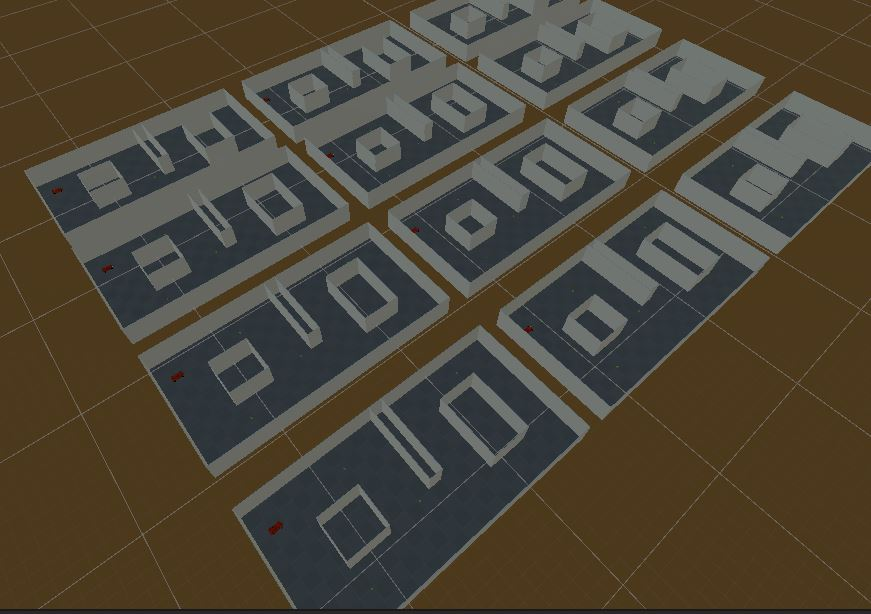
\includegraphics[width=0.9\textwidth]{06_Implementation/00_MLAgents/Images/TrainingMap.JPG}
    \caption[Training Scene]{More instances of the learning environment helps speed up the training.} \label{06:trainingScene}
\end{figure}

% Available models. PPO and SAC. MA-POCA for collab
% Using demonstartion to train faster

%

%continuous vs discrete outputs



%mention attempted checkpoints system.


%\subsection{Collaboration Learning}